\documentclass{article}
\usepackage[utf8]{inputenc}
\usepackage{indentfirst}

\title{\textbf{\underline{Lógica para Computação (IF673)}}}
\author{Lucas Yule Rocha de Melo Araújo}
\date{Outubro, 2019}

\usepackage{natbib}
\usepackage{graphicx}

\begin{document}

\maketitle

\section{\emph{Introdução}}
    A disciplina de lógica para computação busca introduzir as técnicas do \textbf{raciocínio dedutivo} e para isso, se utiliza das ferramentas da \emph{lógica matemática}. A lógica matemática busca estudar e trazer noções acerca dos conceitos de \emph{"consistência,consequencia lógica,validade lógica,decidibilidade,etc,"} de argumentos lógicos. Para tal, também é utilizado elementos da matemática, como \emph{"Teoria dos conjuntos"}e\emph{"algebra booleana"}.\cite{pgDisciplina}

    Na disciplina se estudam:
    \begin{enumerate}
        \item As potencialidades do método formal-dedutivo de representação e raciocínio sobre uma "realidade";
        \item A fundamentação das noções de prova e refutação da validade de argumentos;
        \item Os fundamentos da representação simbólica, e da noção de consequência lógica.
    \end{enumerate}
    
\begin{figure}[h!]
    \centering
    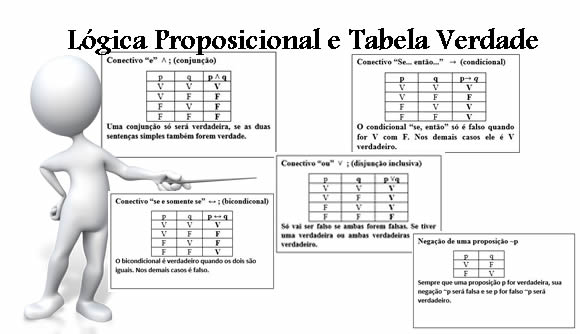
\includegraphics[scale=0.6]{logica.jpeg}
    \caption{Logica proposicional, assunto abordado na disciplina.\cite{imgLogica}}
    \label{fig:my_label}
\end{figure}
\section{\emph{Relevância}}
A relevância da disciplina de \textbf{Lógica para Computação} é tal que, o aluno ao final do período tenha a noção de procedimento efetivo, que deu origem por exemplo à \emph{Máquina de Turing} (primeiro modelo de computador programável por software). O discente também será capaz de mostrar a evolução da lógica, atravez dos trabalhos de \emph{Leibniz, Hilbert e Godel} até culminar no nascimento da ciência da computação através de \emph{Alan Turing}. Além disso o estudante e, futuro profissional da informatica, será munido do conceito de máquina de processamento simbólico e as noções de representação e manipulação simbólica, independente da linguagem utilizada parar a representação.\cite{pgLogica}
\begin{figure}[h!]
    \centering
    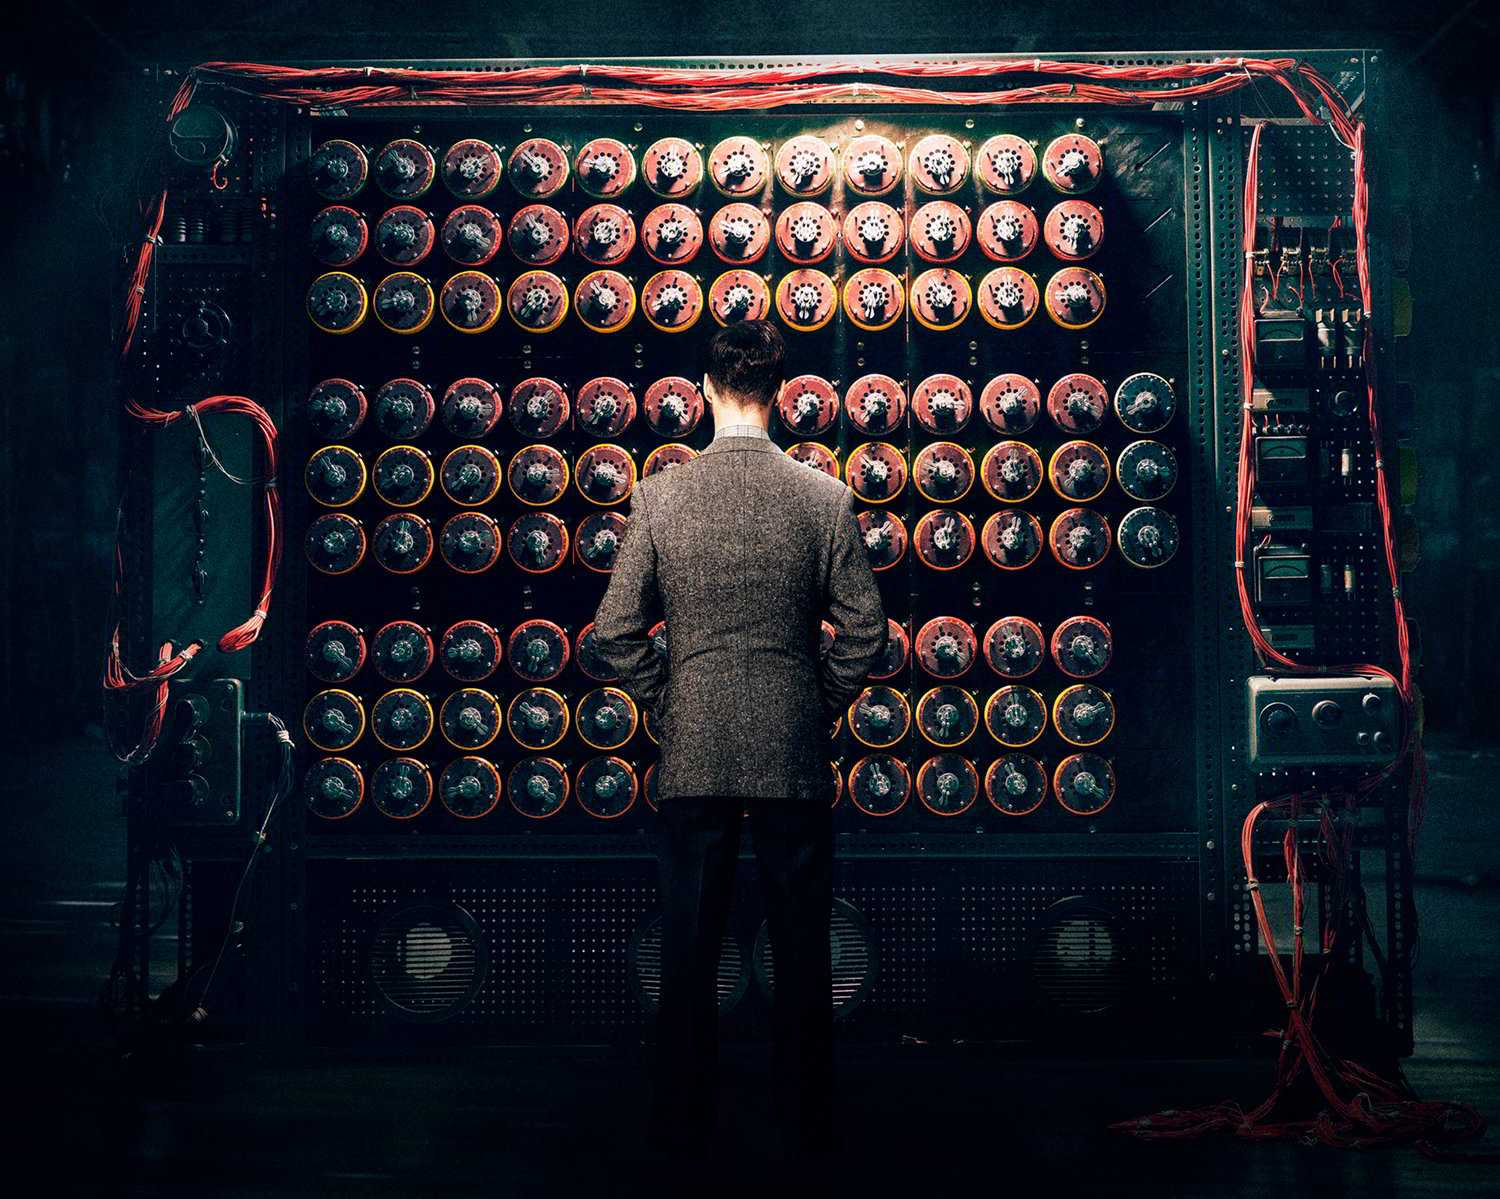
\includegraphics[scale=0.13]{turing.jpg}
    \caption{Maquina de Turing\cite{imgTuring}}
    \label{fig:my_label}
\end{figure}
\section{\emph{Relação com outras disciplinas}}
A disciplina de \textbf{lógica para computação} se relaciona amplamente com a disciplina \textbf{matemática discreta}, uma vez que ambas se nutrem do raciocínio lógico e buscam manipular e utilizar os principais conceitos de lógica proposicional, relações, consequencias lógicas e métodos de prova.

\bibliographystyle{plain}
\bibliography{lyrma}
\end{document}
